% -*- program:xelatex -*-

\documentclass[12pt]{beamer}

\usetheme{metropolis}

\usepackage{fancyvrb}
\usepackage{soul}
\usepackage{booktabs}
\usepackage{multirow}
\usepackage{multicol}
\usepackage{minted}
\usepackage{hyperref}
\usepackage[export]{adjustbox}

\title{Statistical Computing as an Introduction to Data Science}
\subtitle{}
\date{JSM 2016 - Chicago}
\author{Colin Rundel}
\institute{Duke University\\Department of Statistical Science}
% \titlegraphic{\hfill\includegraphics[height=1.5cm]{logo/logo}}

\begin{document}

\maketitle

%%%%%%%%%%%%%%%%%%%%%%%%%%%%%%%%%%%%%%%%%%%%%%%%%%%%%%%%%%%%%%%%%%%%%%%%%%%%%%

\begin{frame}
\frametitle{Sta 323 - Statistical Computing}

Course details:
\begin{itemize}
\item Foundational computing course
\vspace{2mm}
\item 2nd/3rd year elective for BSS
\vspace{2mm}
\item Approximately 40 Students divided into teams of 4
\vspace{2mm}
\item Biweekly team programming assignments
\vspace{2mm}
\item Individual take-home midterms, team final project
\end{itemize}

\end{frame}

%%%%%%%%%%%%%%%%%%%%%%%%%%%%%%%%%%%%%%%%%%%%%%%%%%%%%%%%%%%%%%%%%%%%%%%%%%%%%%

\begin{frame}
\frametitle{Learning Objectives}

{\large
\begin{enumerate}
 
\item R programming and ecosystem \\
      \begin{center} {\small (R + Tidyverse)} \end{center}

\vspace{5mm}

\item Reproducible Research \\
      \begin{center} {\small (rmarkdown + knitr + \emph{make})} \end{center}

\vspace{5mm}

\item Software Engineering / Collaboration \\
      \begin{center} {\small (shell + git + github)} \end{center}

\end{enumerate}
}
\end{frame}

%%%%%%%%%%%%%%%%%%%%%%%%%%%%%%%%%%%%%%%%%%%%%%%%%%%%%%%%%%%%%%%%%%%%%%%%%%%%%%

\begin{frame}
\frametitle{Infrastructure}

Dedicated departmental server
\begin{itemize}
\item RStudio Server Pro
\item Individual departmental accounts
\item System wide install of default packages
\end{itemize}

\vspace{3mm}

Github Organization
\begin{itemize}
\item 1 Organization / class
\item 1 private repo / team / assignment
\item Shared public repos (e.g. examples)
\item CI / Testing via Wercker
\end{itemize}

\end{frame}


%%%%%%%%%%%%%%%%%%%%%%%%%%%%%%%%%%%%%%%%%%%%%%%%%%%%%%%%%%%%%%%%%%%%%%%%%%%%%%

\begin{frame}
\frametitle{Why github?}

All assignment (and project) related work is maintained on github 

\vspace{1.5mm}

\begin{itemize}
\item Forces students to use version control (git)
\item Simplifies course administration
\begin{itemize}
\item Code / documentation / scaffolding in one place
\item Easy to grab files (pull)
\item Easy to distribute files (push)
\item Built-in team permissions
\end{itemize}
\item Searchability
\item Accountability
\item Continuous integration tools
\end{itemize}

\end{frame}

%%%%%%%%%%%%%%%%%%%%%%%%%%%%%%%%%%%%%%%%%%%%%%%%%%%%%%%%%%%%%%%%%%%%%%%%%%%%%%

\begin{frame}[t]
\frametitle{Course Sketch}

\begin{enumerate}

\item[]
    
\begin{enumerate}

\item[\qquad HW1 - ] FizzBuzz {\scriptsize(Workflow basics)}

~\\

\item[\qquad HW2 - ] Graph Data Structures {\scriptsize(Base R, testing)}

~\\

\item[\qquad HW3 - ] La Quinta is Spanish for next to Denny's \\ {\scriptsize(Web APIs, scraping, make)}

~\\

\item[\qquad HW4 - ] Karl Broman's Socks {\scriptsize(Shiny, profiling, parallelization)}

~\\

\item[\qquad HW5 - ] Parking Wars: Manhattan {\scriptsize(Data munging, prediction)}

~\\

\item[\qquad HW6 - ] How big is your data? {\scriptsize(Hadoop, Spark)}

\end{enumerate}

\end{enumerate}
    
\end{frame}

%%%%%%%%%%%%%%%%%%%%%%%%%%%%%%%%%%%%%%%%%%%%%%%%%%%%%%%%%%%%%%%%%%%%%%%%%%%%%%

\begin{frame}[t]
\frametitle{HW3 - La Quinta is Spanish for next to Denny's}

\makebox[\linewidth][c]{
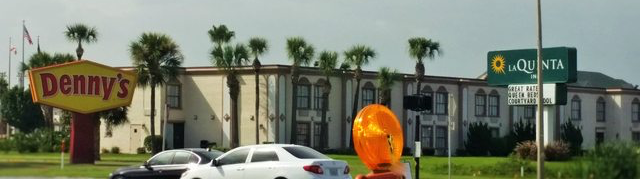
\includegraphics[width=\textwidth]{imgs/dennys_lq_signs.png}
}

\vspace{5mm}

Assignment is based on a \href{http://njgeo.org/2014/01/30/mitch-hedberg-and-gis/}{post} by John Reiser on his \href{http://njgeo.org/}{new jersey geographer blog}.

\vspace{5mm}

See Taking a Chance in the Classroom (Chance Vol. 29, Iss. 2, 2016) for a more detailed write up the statistical analysis aspect of this assignment.

\end{frame}

%%%%%%%%%%%%%%%%%%%%%%%%%%%%%%%%%%%%%%%%%%%%%%%%%%%%%%%%%%%%%%%%%%%%%%%%%%%%%%

\begin{frame}[t]
\frametitle{Finding Denny's Locations}

\makebox[\linewidth][c]{
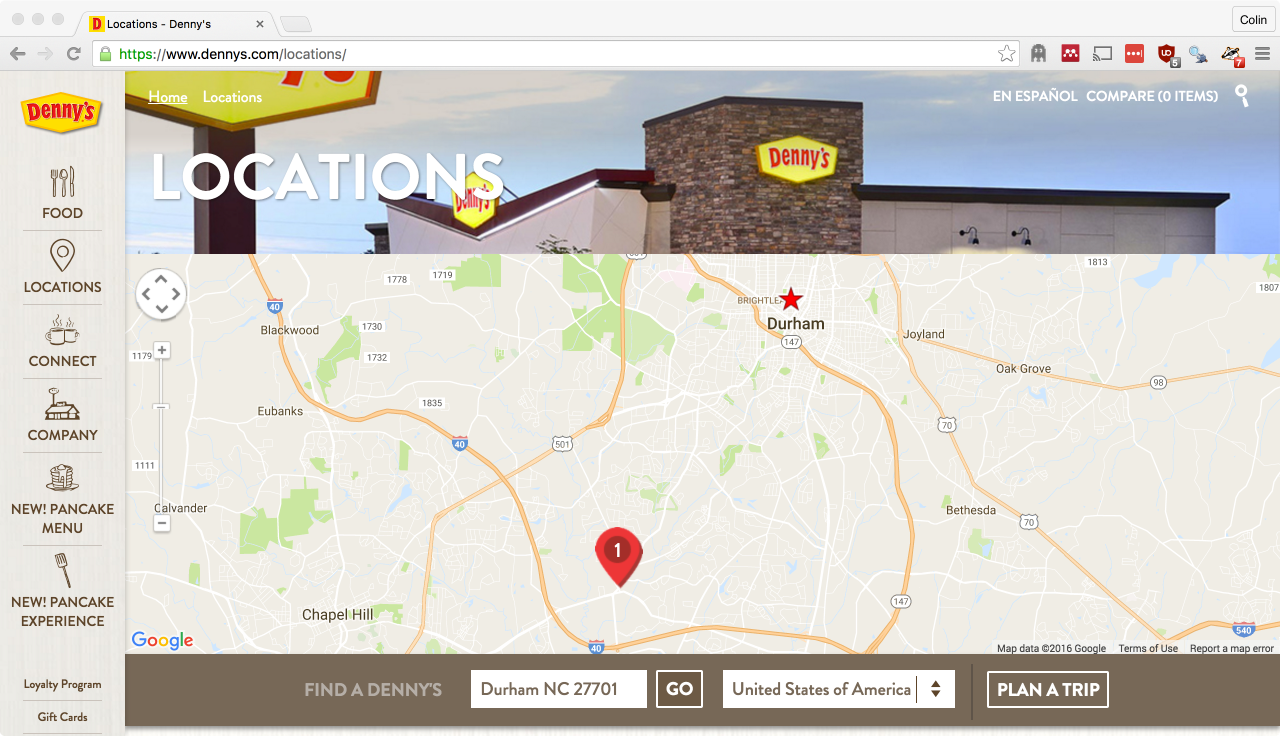
\includegraphics[width=1.10\textwidth]{imgs/dennys_website.png}
}

\end{frame}


%%%%%%%%%%%%%%%%%%%%%%%%%%%%%%%%%%%%%%%%%%%%%%%%%%%%%%%%%%%%%%%%%%%%%%%%%%%%%%

\begin{frame}[t]
\frametitle{Finding the API}

\makebox[\linewidth][c]{
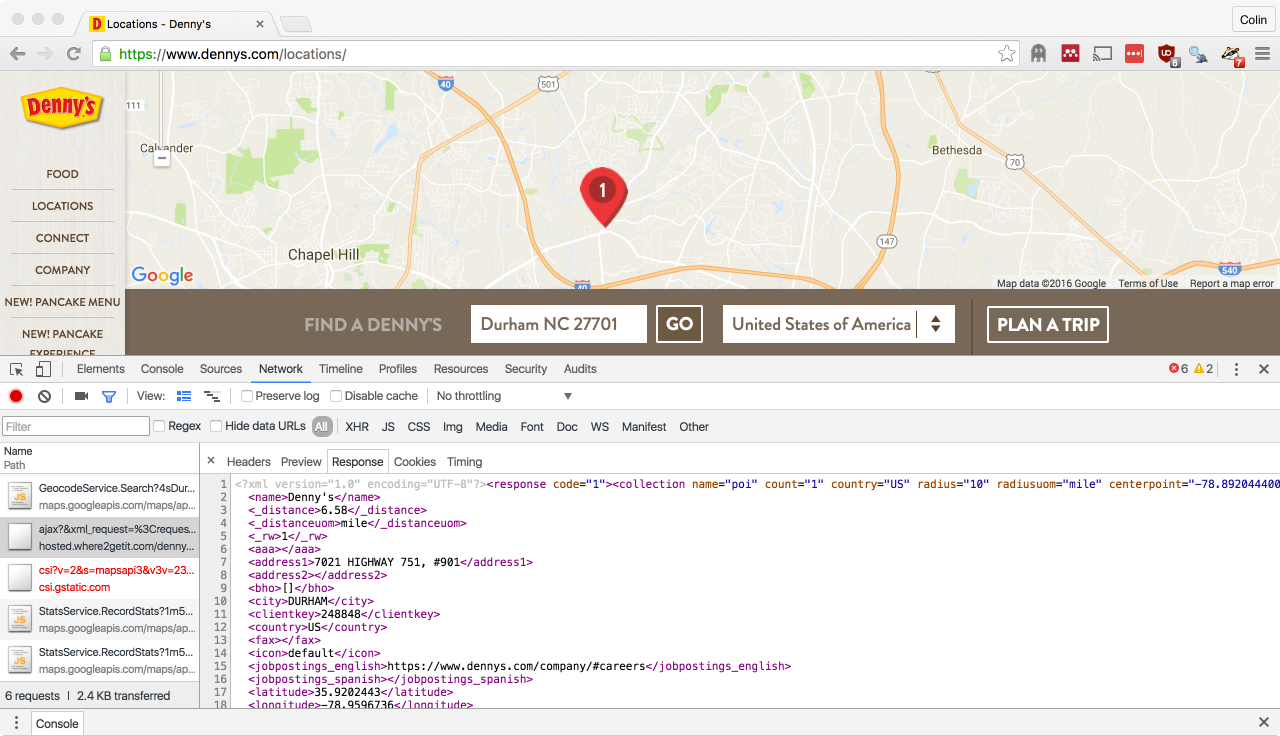
\includegraphics[width=1.10\textwidth]{imgs/dennys_xml.png}
}

\end{frame}

%%%%%%%%%%%%%%%%%%%%%%%%%%%%%%%%%%%%%%%%%%%%%%%%%%%%%%%%%%%%%%%%%%%%%%%%%%%%%%

% \begin{frame}[fragile]
% \frametitle{API Results}

% {\tiny
% \begin{minted}[breaklines]{xml}
% <response code="1">
%   <collection name="poi" count="1" country="US" radius="10" radiusuom="mile" centerpoint="-78.89204440000003,35.9981205" state="NC"       city="Durham" address="" province="" postalcode="27701">
%     <poi>
%       <name>Denny's</name>
%       <_distance>6.58</_distance>
%       <_distanceuom>mile</_distanceuom>
%       <_rw>1</_rw>
%       <aaa/>
%       <address1>7021 HIGHWAY 751, #901</address1>
%       <address2/>
%       <bho>[]</bho>
%       <city>DURHAM</city>
%       <clientkey>248848</clientkey>
%       <country>US</country>
%       <fax/>
%       <icon>default</icon>
%       <jobpostings_english>https://www.dennys.com/company/#careers</jobpostings_english>
%       <jobpostings_spanish/>
%       <latitude>35.9202443</latitude>
%       <longitude>-78.9596736</longitude>
%       <loyalty_program/>
%       <onlineordering/>
%       <other>8848</other>
%       <phone>(919) 908-1006</phone>
%       <postalcode>27707</postalcode>
%       <province/>
%       <rank/>
%       <state>NC</state>
%       <status>0</status>
%       <travelplaza>0</travelplaza>
%       <uid>1921743355</uid>
%     </poi>
%   </collection>
% </response>
% \end{minted}
% }

% \end{frame}

%%%%%%%%%%%%%%%%%%%%%%%%%%%%%%%%%%%%%%%%%%%%%%%%%%%%%%%%%%%%%%%%%%%%%%%%%%%%%%

\begin{frame}[fragile]
\frametitle{API Request}

%https://hosted.where2getit.com/dennys/responsive/ajax?&xml_request=<request><appkey>6B962D40-03BA-11E5-BC31-9A51842CA48B</appkey><formdata id="locatorsearch"><dataview>store_default</dataview><limit>16</limit><order>rank,_distance</order><geolocs><geoloc><addressline>Durham NC 27701</addressline><longitude>-78.89204440000003</longitude><latitude>35.9981205</latitude><country>US</country></geoloc></geolocs><stateonly>1</stateonly><searchradius>10|25|50|100</searchradius></formdata></request>

{\scriptsize

\begin{Verbatim}
https://hosted.where2getit.com/dennys/responsive/ajax?&xml_request=
<request>
<appkey>6B962D40-03BA-11E5-BC31-9A51842CA48B</appkey>
    <formdata id="locatorsearch">
        <dataview>store_default</dataview>
        <limit>16</limit>
        <order>rank,_distance</order>
        <geolocs>
            <geoloc>
                <addressline>Durham NC 27701</addressline>
                <longitude>-78.89204440000003</longitude>
                <latitude>35.9981205</latitude>
                <country>US</country>
            </geoloc>
        </geolocs>
        <stateonly>1</stateonly>
        <searchradius>10|25|50|100</searchradius>
    </formdata>
</request>
\end{Verbatim}
}

\end{frame}

%%%%%%%%%%%%%%%%%%%%%%%%%%%%%%%%%%%%%%%%%%%%%%%%%%%%%%%%%%%%%%%%%%%%%%%%%%%%%%

\begin{frame}[fragile]
\frametitle{API Request}

{\scriptsize
\begin{Verbatim}[commandchars=\\\{\}]
https://hosted.where2getit.com/dennys/responsive/ajax?&xml_request=
<request>
<appkey>6B962D40-03BA-11E5-BC31-9A51842CA48B</appkey>
    <formdata id="locatorsearch">
        <dataview>store_default</dataview>
        \hl{<limit>16</limit>}
        <order>rank,_distance</order>
        <geolocs>
            <geoloc>
                <addressline>Durham NC 27701</addressline>
                \hl{<longitude>-78.89204440000003</longitude>}
                \hl{<latitude>35.9981205</latitude>}
                <country>US</country>
            </geoloc>
        </geolocs>
        <stateonly>1</stateonly>
        \hl{<searchradius>10|25|50|100</searchradius>}
    </formdata>
</request>
\end{Verbatim}
}

\end{frame}


%%%%%%%%%%%%%%%%%%%%%%%%%%%%%%%%%%%%%%%%%%%%%%%%%%%%%%%%%%%%%%%%%%%%%%%%%%%%%%

\begin{frame}[t]
\frametitle{API Results}

\vspace{-3mm}

\begin{center}
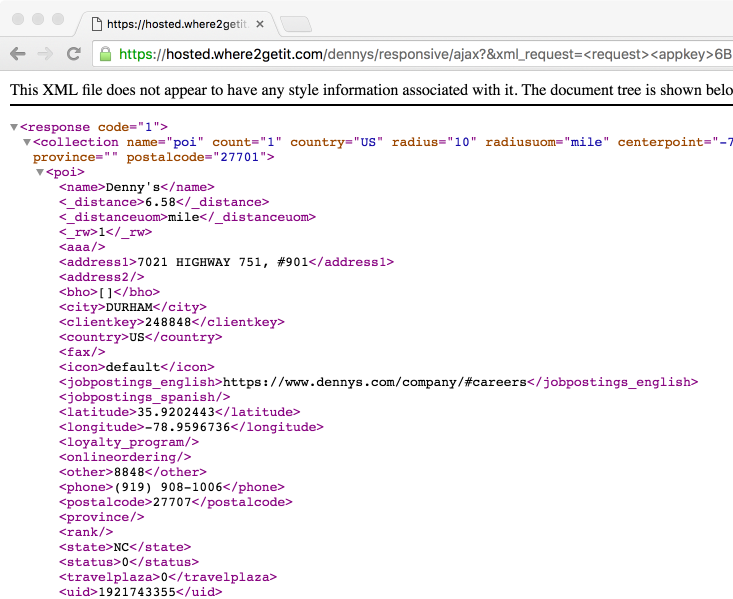
\includegraphics[width=0.9\textwidth]{imgs/dennys_xml_page.png}
\end{center}

\end{frame}

%%%%%%%%%%%%%%%%%%%%%%%%%%%%%%%%%%%%%%%%%%%%%%%%%%%%%%%%%%%%%%%%%%%%%%%%%%%%%%

\begin{frame}[t]
\frametitle{Finding La Quinta Locations}

\begin{center}
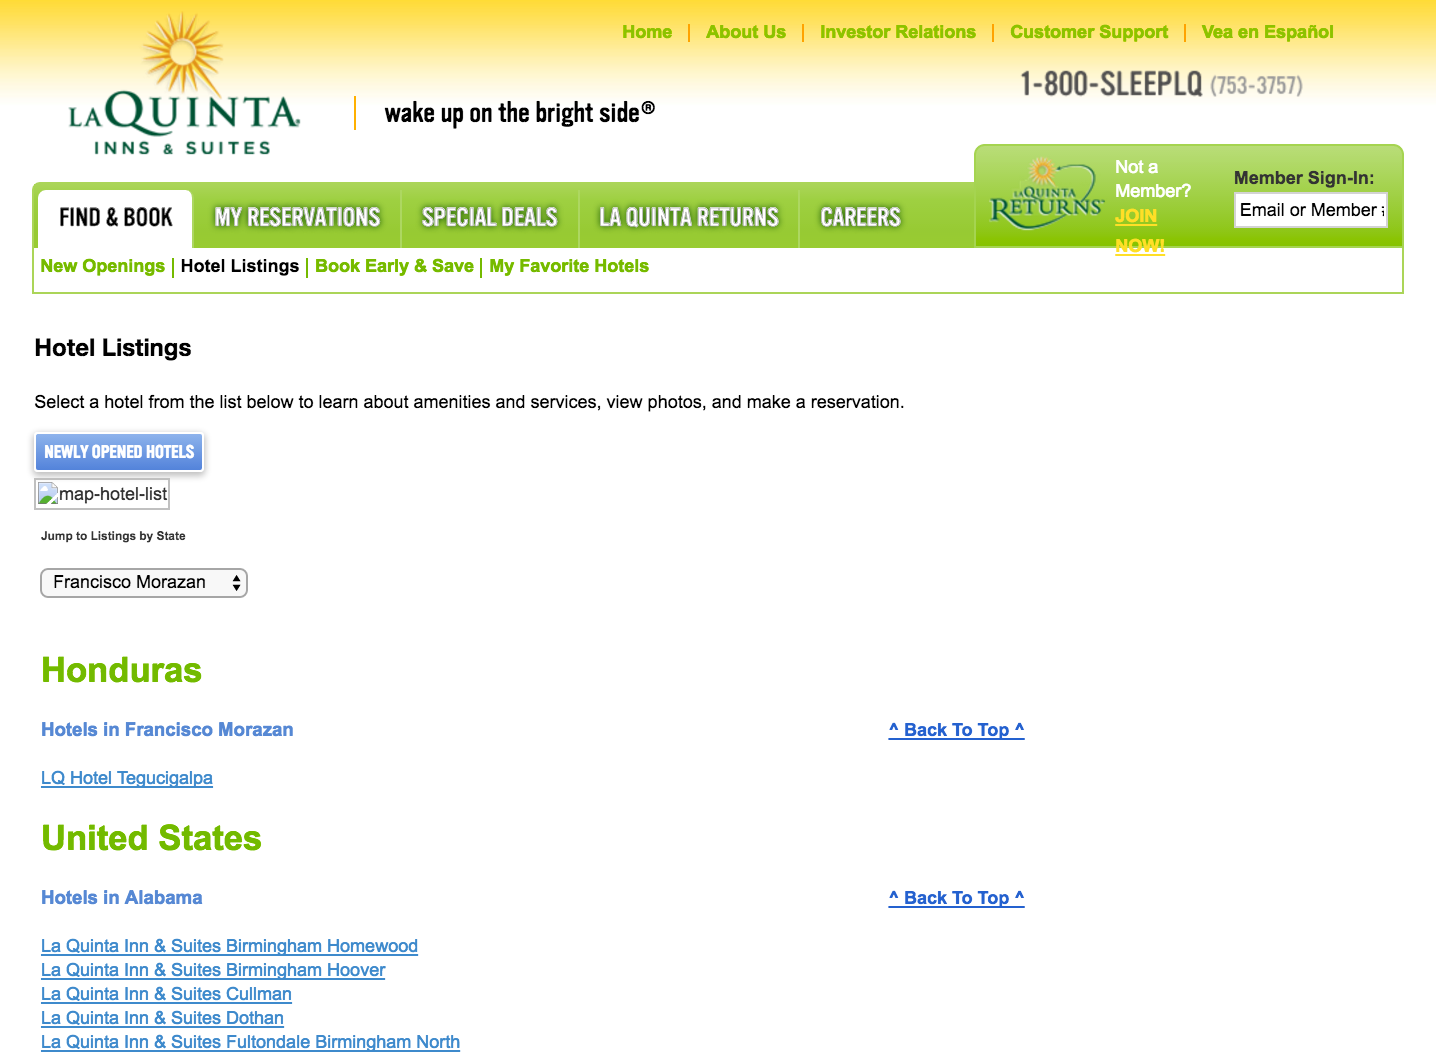
\includegraphics[width=0.9\textwidth]{imgs/lq_listings.png}
\end{center}

\end{frame}


%%%%%%%%%%%%%%%%%%%%%%%%%%%%%%%%%%%%%%%%%%%%%%%%%%%%%%%%%%%%%%%%%%%%%%%%%%%%%%

\begin{frame}[t]
\frametitle{Finding La Quinta Location Information}

\vspace{-4mm}

\begin{center}
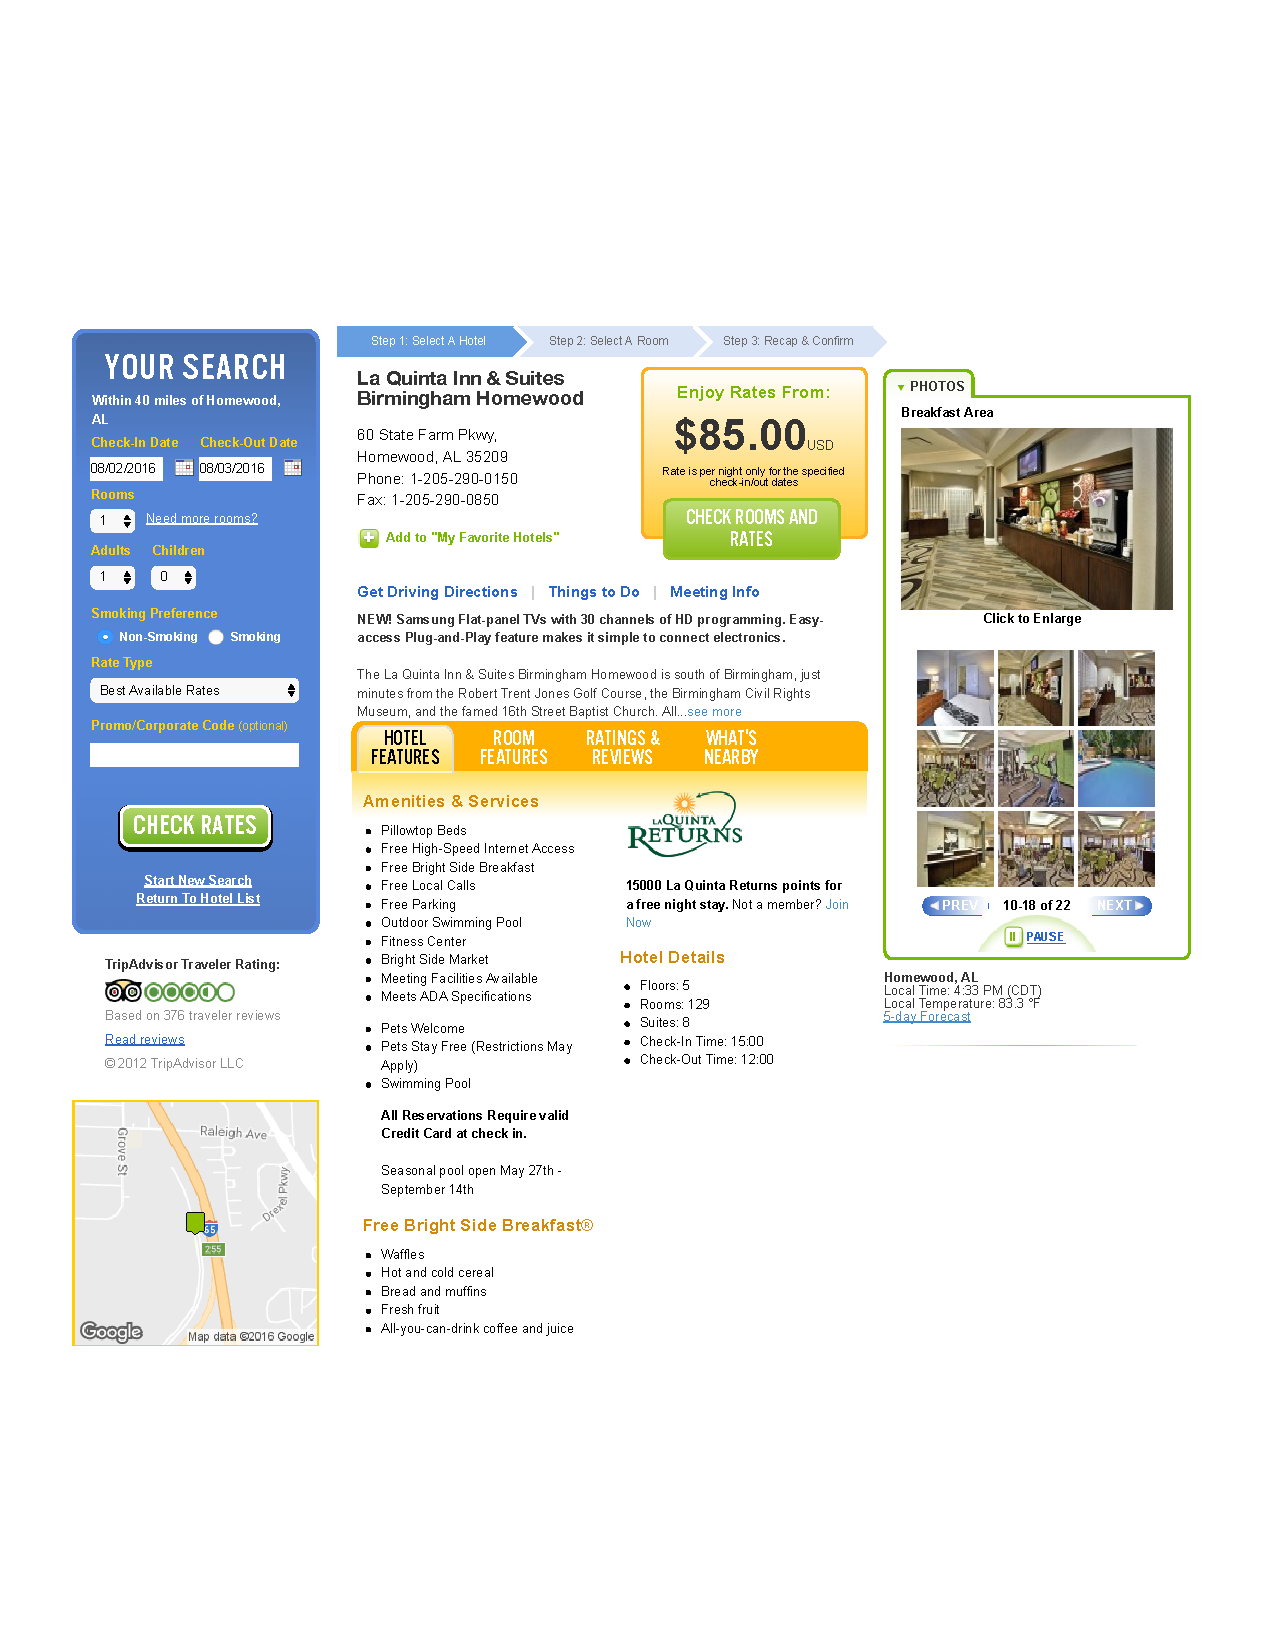
\includegraphics[width=0.9\textwidth]{imgs/lq_hotel_page.pdf}
\end{center}

\end{frame}

%%%%%%%%%%%%%%%%%%%%%%%%%%%%%%%%%%%%%%%%%%%%%%%%%%%%%%%%%%%%%%%%%%%%%%%%%%%%%%

\begin{frame}[t]
\frametitle{Reproducibility}

{\small
Up to this point all reproducibility is based on individual Rmd documents (code and analysis in the same place)

\begin{itemize}
\pause \item Not feasible for this task - (irresponsible) grabbing of Denny's and La Quinta pages takes several minutes.

\pause \item This is a ``solved'' problem for software development - build tools (e.g. make)
\end{itemize}
}

\pause

\vspace{-2mm}
\makebox[\linewidth][c]{
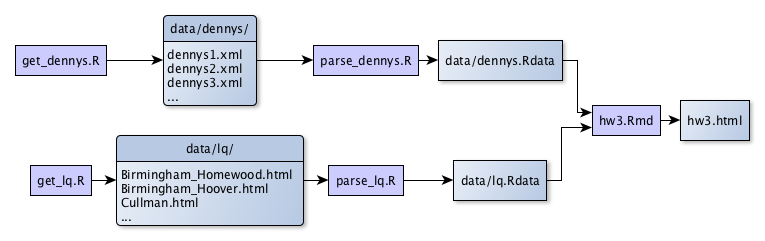
\includegraphics[width=1.1\textwidth]{imgs/HW3_Makefile.png}
}

\end{frame}


%%%%%%%%%%%%%%%%%%%%%%%%%%%%%%%%%%%%%%%%%%%%%%%%%%%%%%%%%%%%%%%%%%%%%%%%%%%%%%

\begin{frame}
\frametitle{Github Repo}

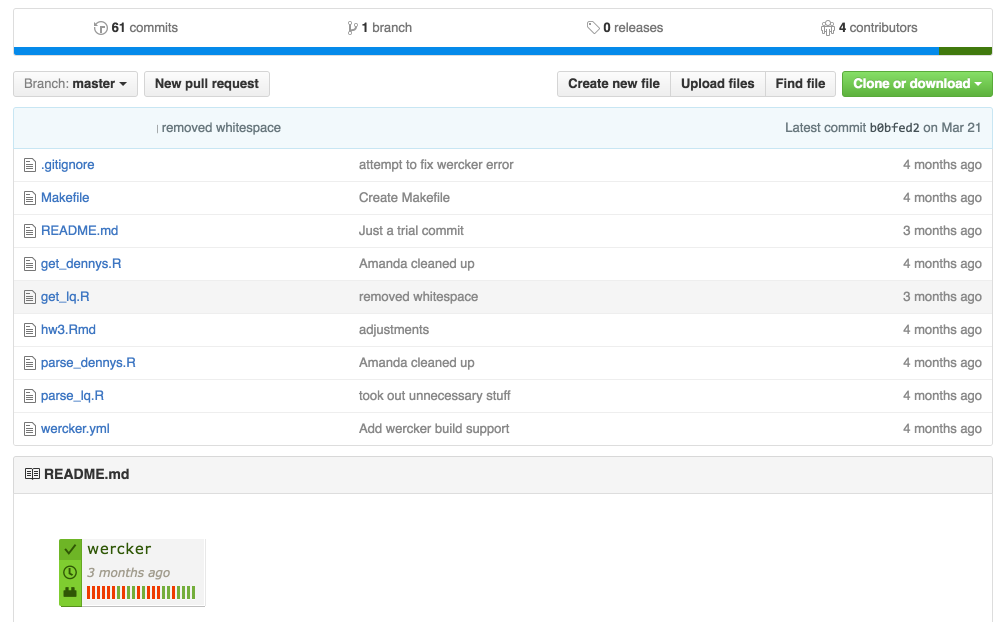
\includegraphics[width=\textwidth]{imgs/github_repo.png}
    
\end{frame}

%%%%%%%%%%%%%%%%%%%%%%%%%%%%%%%%%%%%%%%%%%%%%%%%%%%%%%%%%%%%%%%%%%%%%%%%%%%%%%

\begin{frame}
\frametitle{Github Commits}

\makebox[\linewidth][c]{
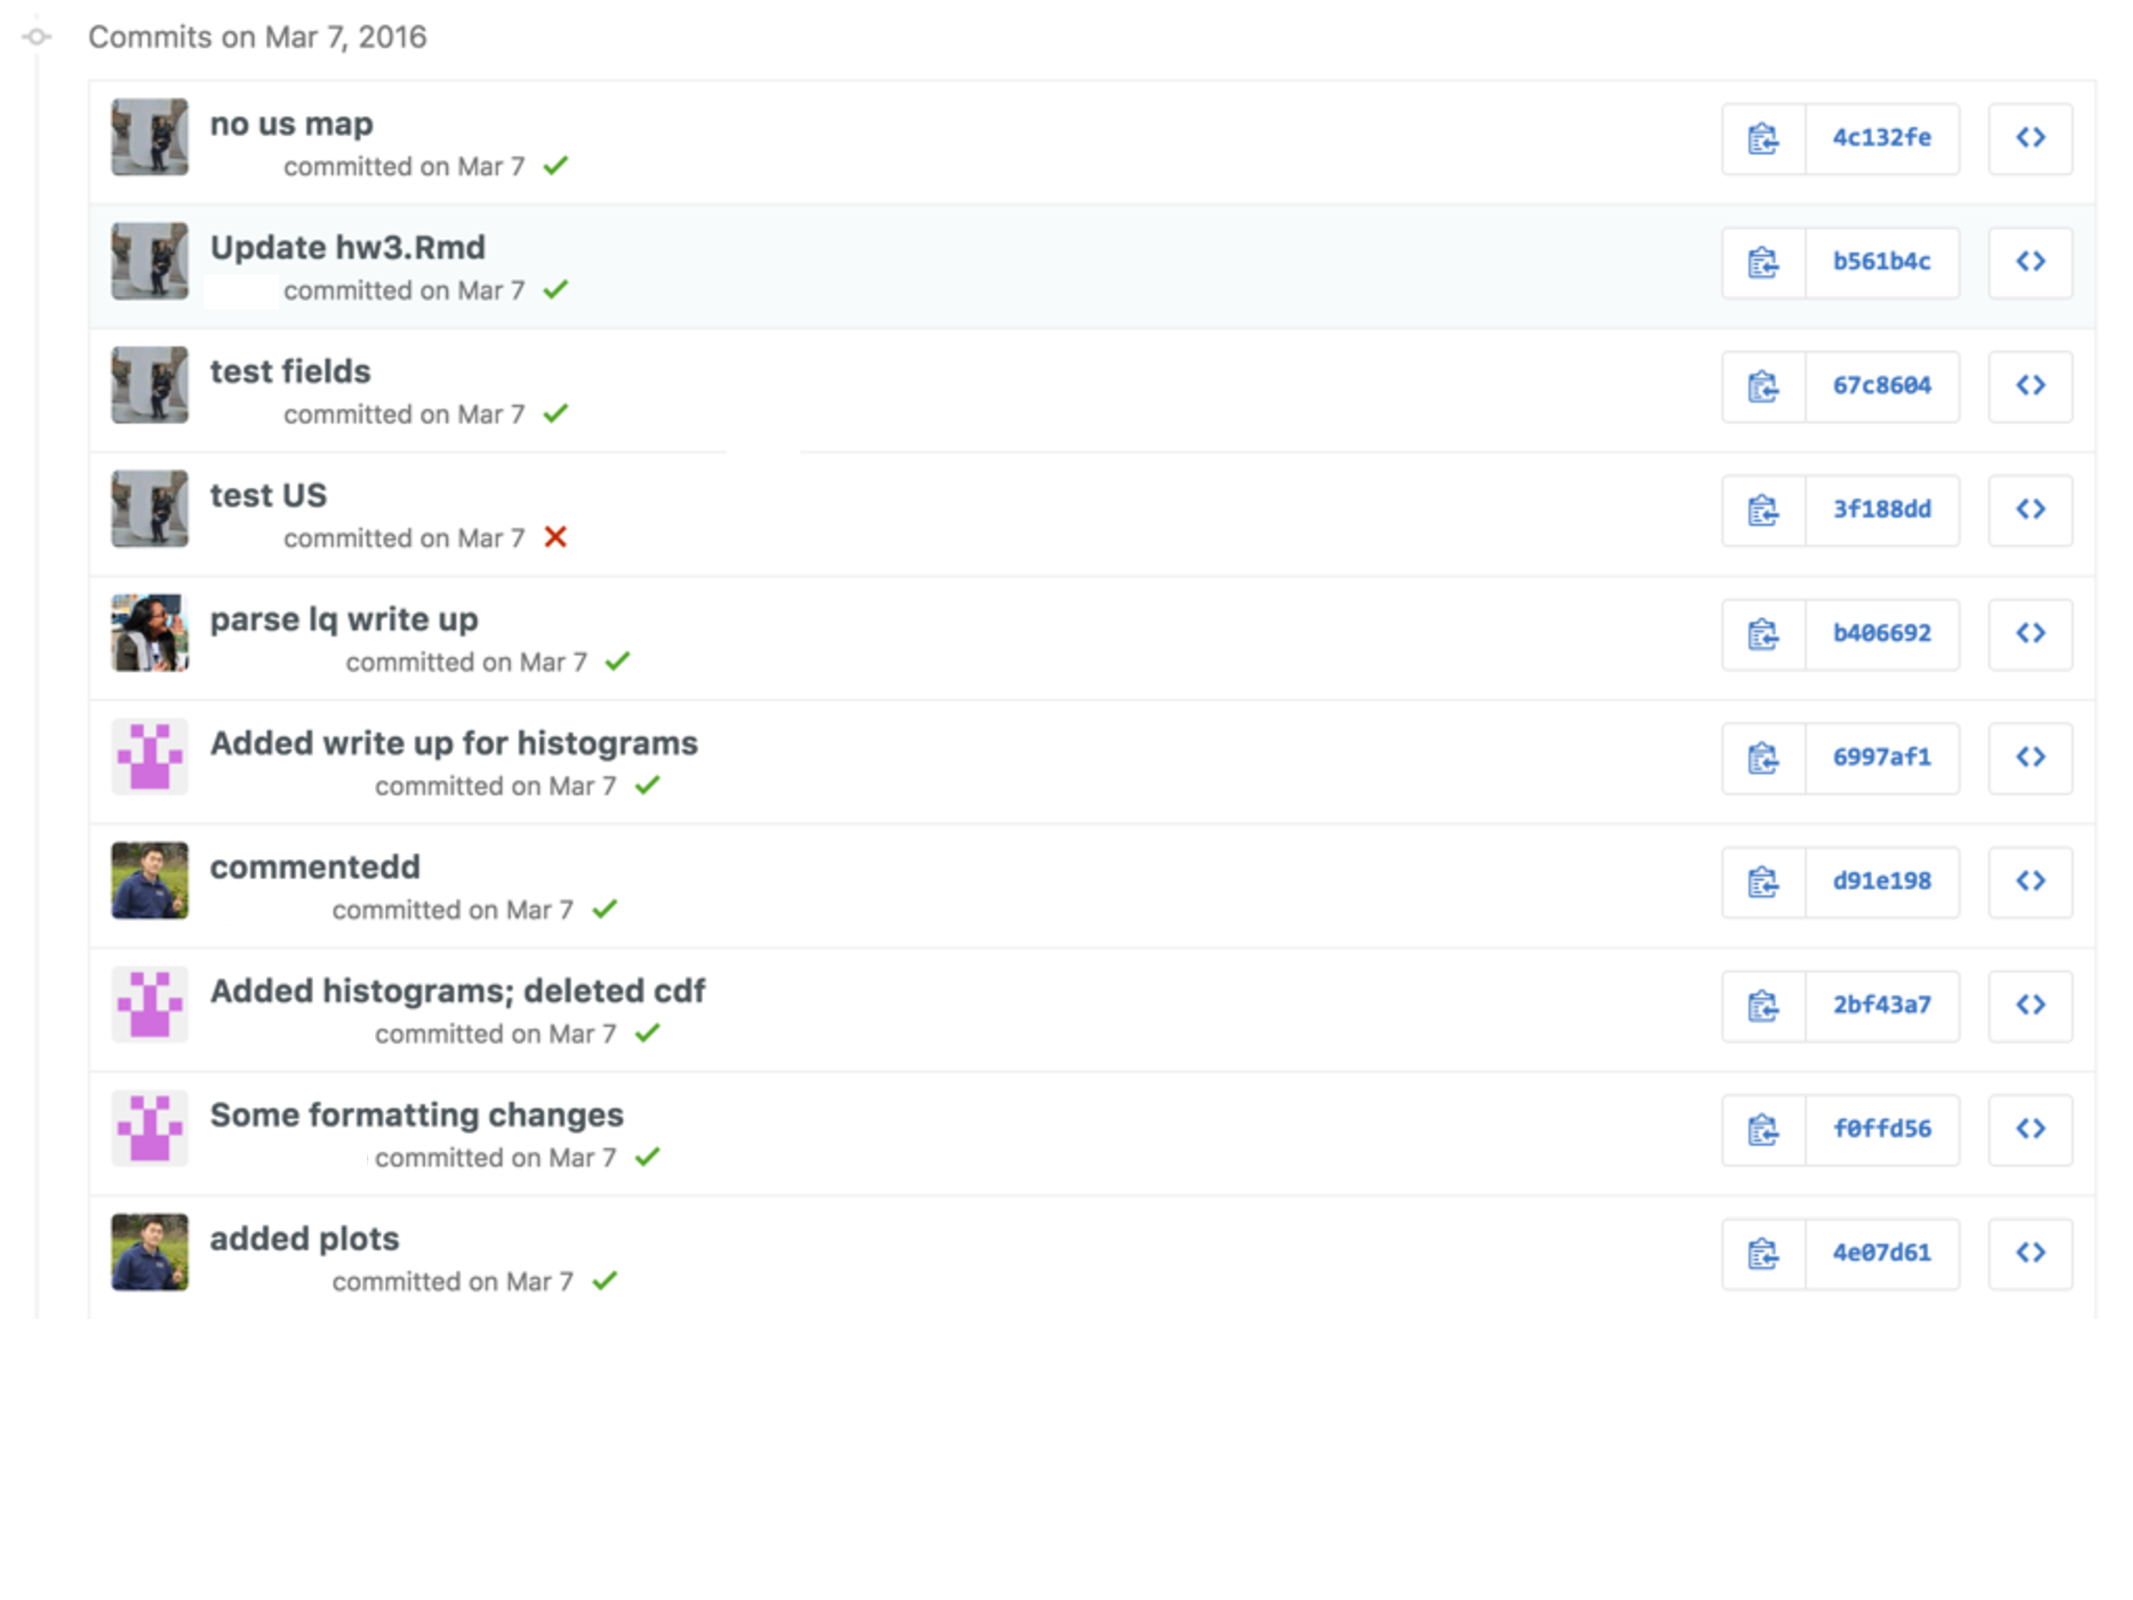
\includegraphics[width=1.1\textwidth]{imgs/github_commits.pdf}
}

\end{frame}

%%%%%%%%%%%%%%%%%%%%%%%%%%%%%%%%%%%%%%%%%%%%%%%%%%%%%%%%%%%%%%%%%%%%%%%%%%%%%%

\begin{frame}
\frametitle{Feedback loop}

\begin{center}
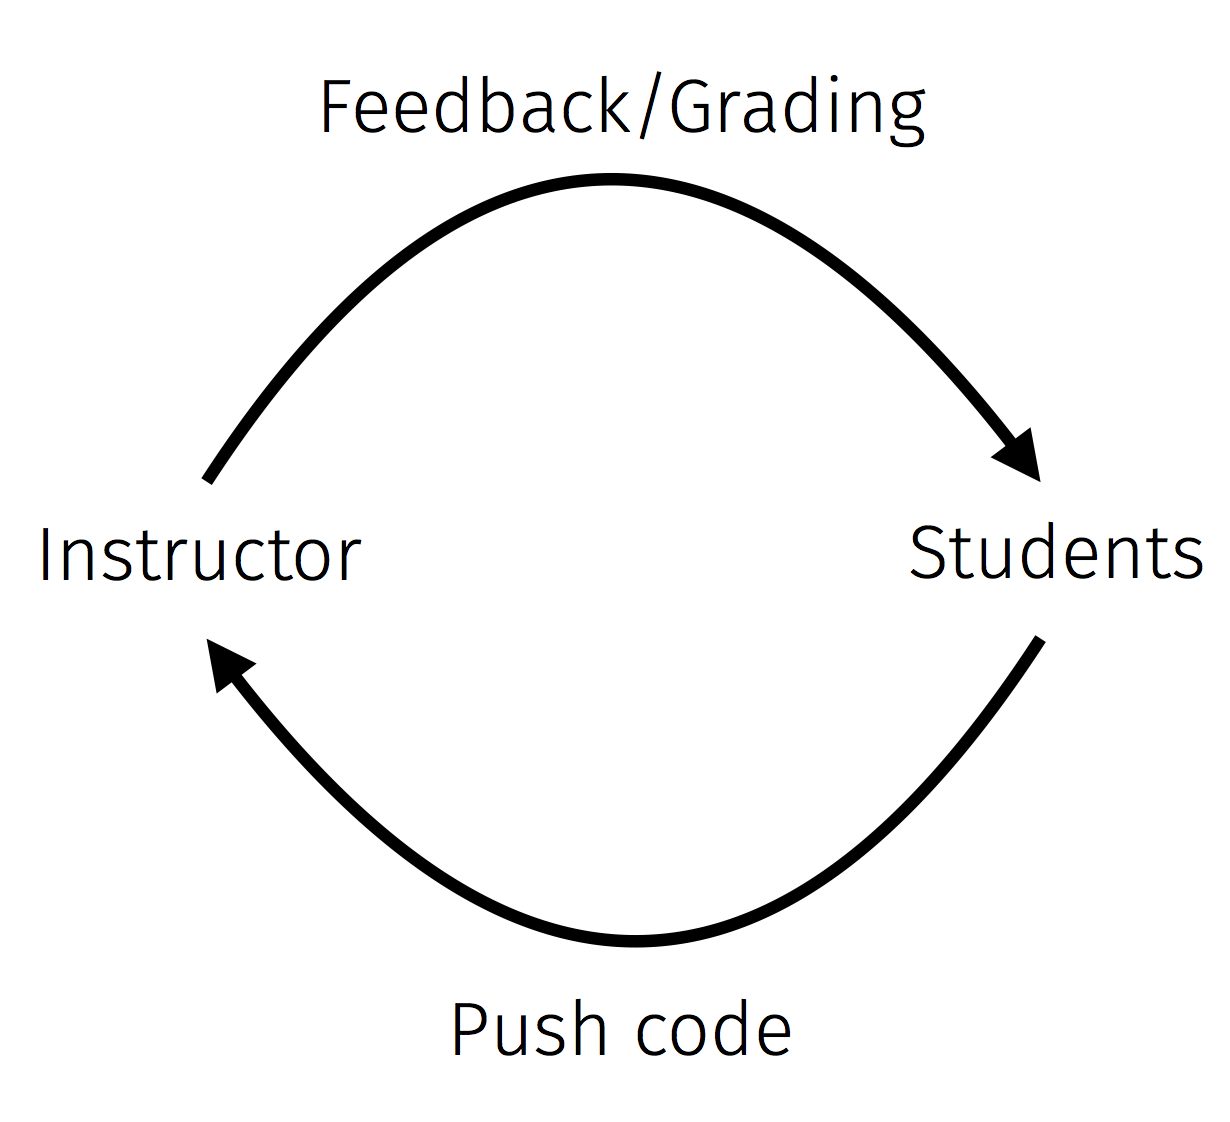
\includegraphics[width=0.5\textwidth]{imgs/cycle.png}
\end{center}

\pause

Github is great for feedback and accountability but doesn't address scalability of the instructor and TAs (we are the rate limiting step).

\end{frame}

%%%%%%%%%%%%%%%%%%%%%%%%%%%%%%%%%%%%%%%%%%%%%%%%%%%%%%%%%%%%%%%%%%%%%%%%%%%%%%

\begin{frame}[fragile]
\frametitle{A painfully common conversation}

{\footnotesize
\textit{Student: We've submitted HW3!}
%
\begin{center} +1 Day \end{center}
%
\textit{Me: Your Rmd file doesn't knit, you used \mintinline{r}{setwd} with an absolute path.}
%
\begin{center} +1 Day \end{center}
%
\textit{Student: Ok we fixed that, does it work now?}
%
\begin{center} +1 Day \end{center}
%
\textit{Me: Nope, you used \mintinline{r}{lme4} without checking if it was installed.}
%
\begin{center} +1 Day \end{center}
%
\begin{center} $\vdots$ \end{center}
}
\end{frame}

%%%%%%%%%%%%%%%%%%%%%%%%%%%%%%%%%%%%%%%%%%%%%%%%%%%%%%%%%%%%%%%%%%%%%%%%%%%%%%

\begin{frame}
\frametitle{Course Process Cartoon - Improved}

\begin{center}
%\only<1>{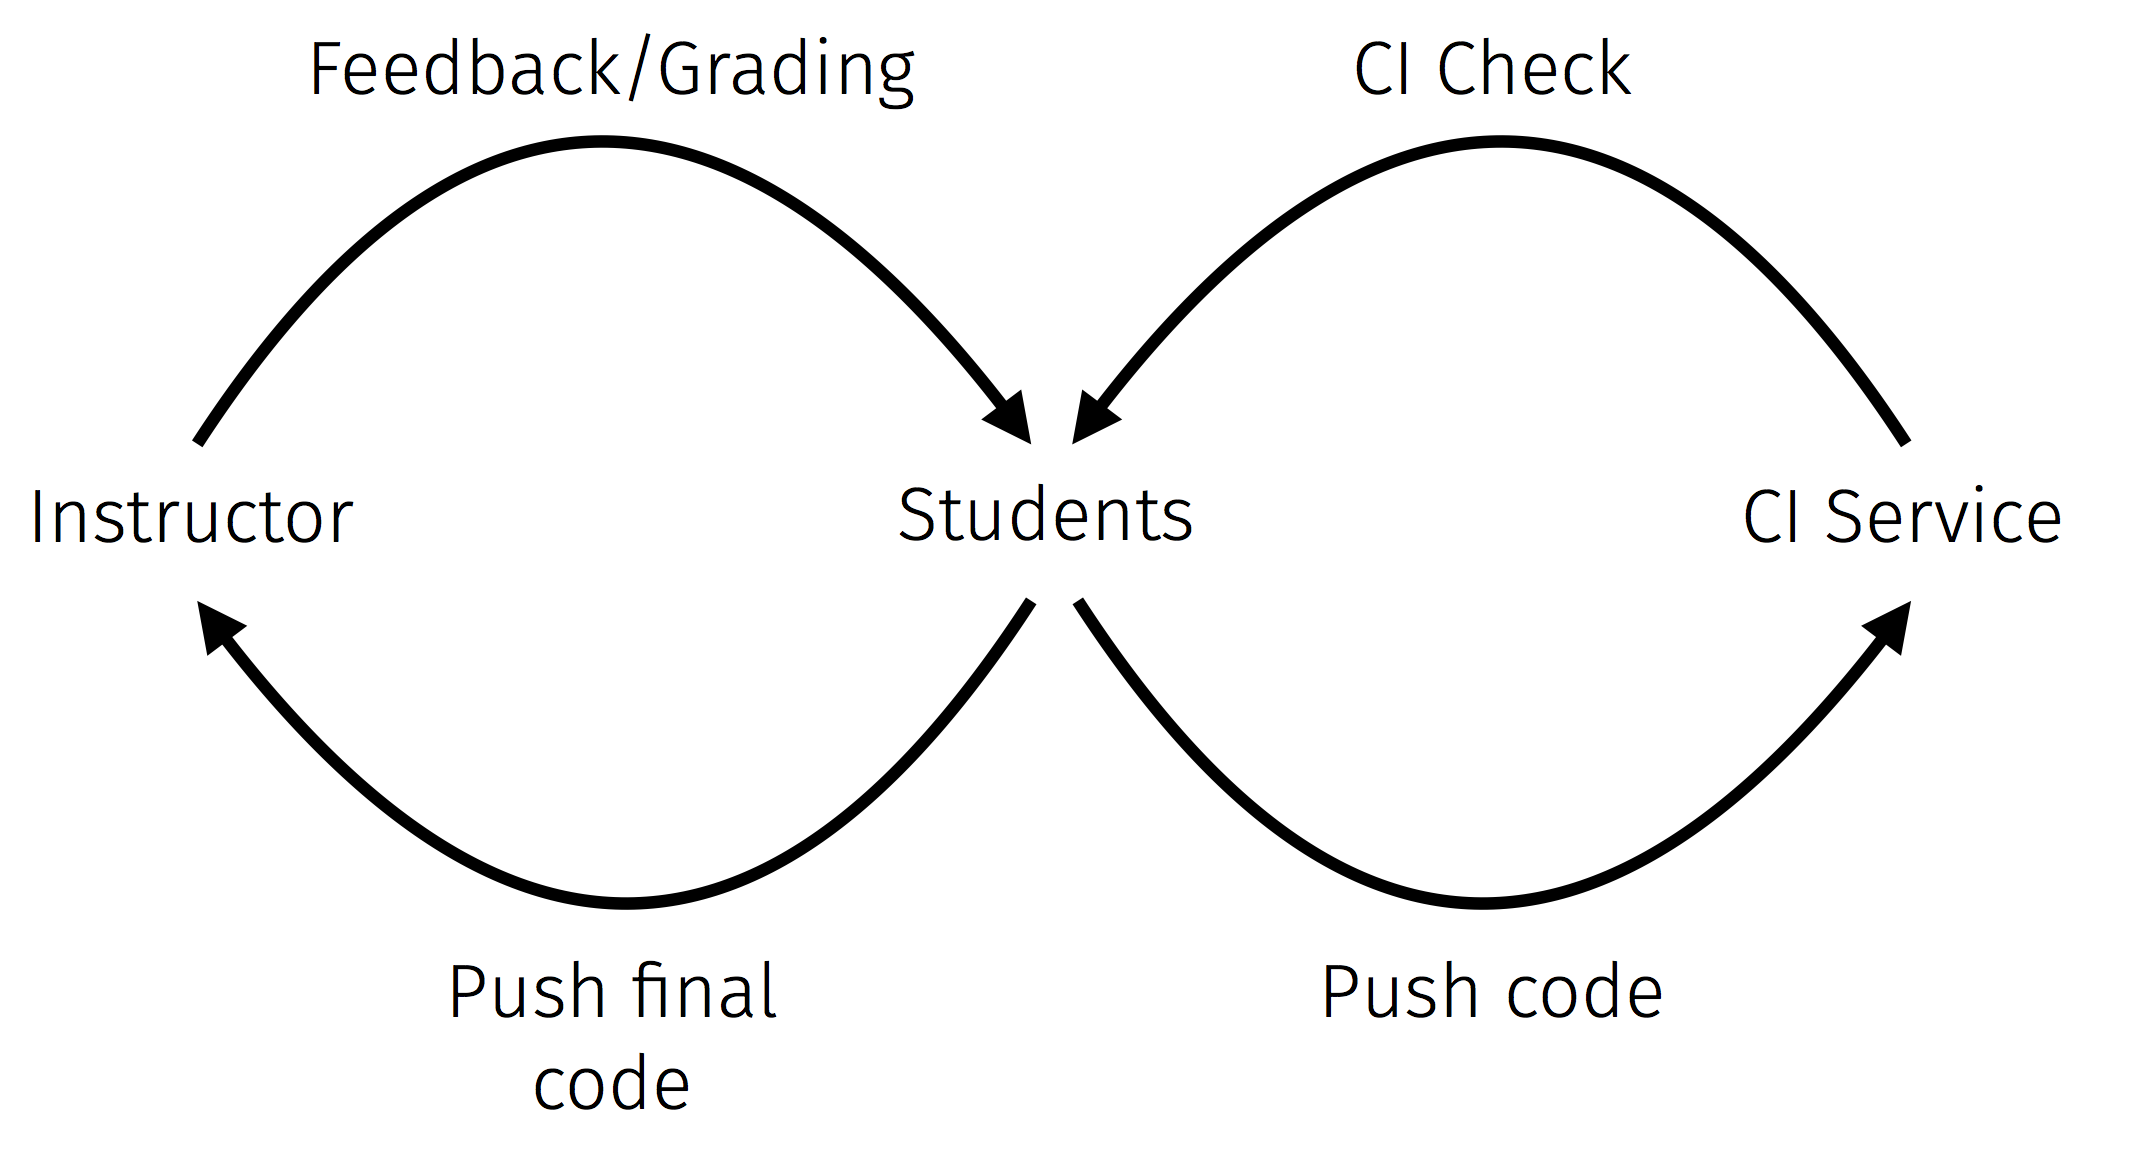
\includegraphics[width=\textwidth]{imgs/cycle_ci.png}}
%\only<2>{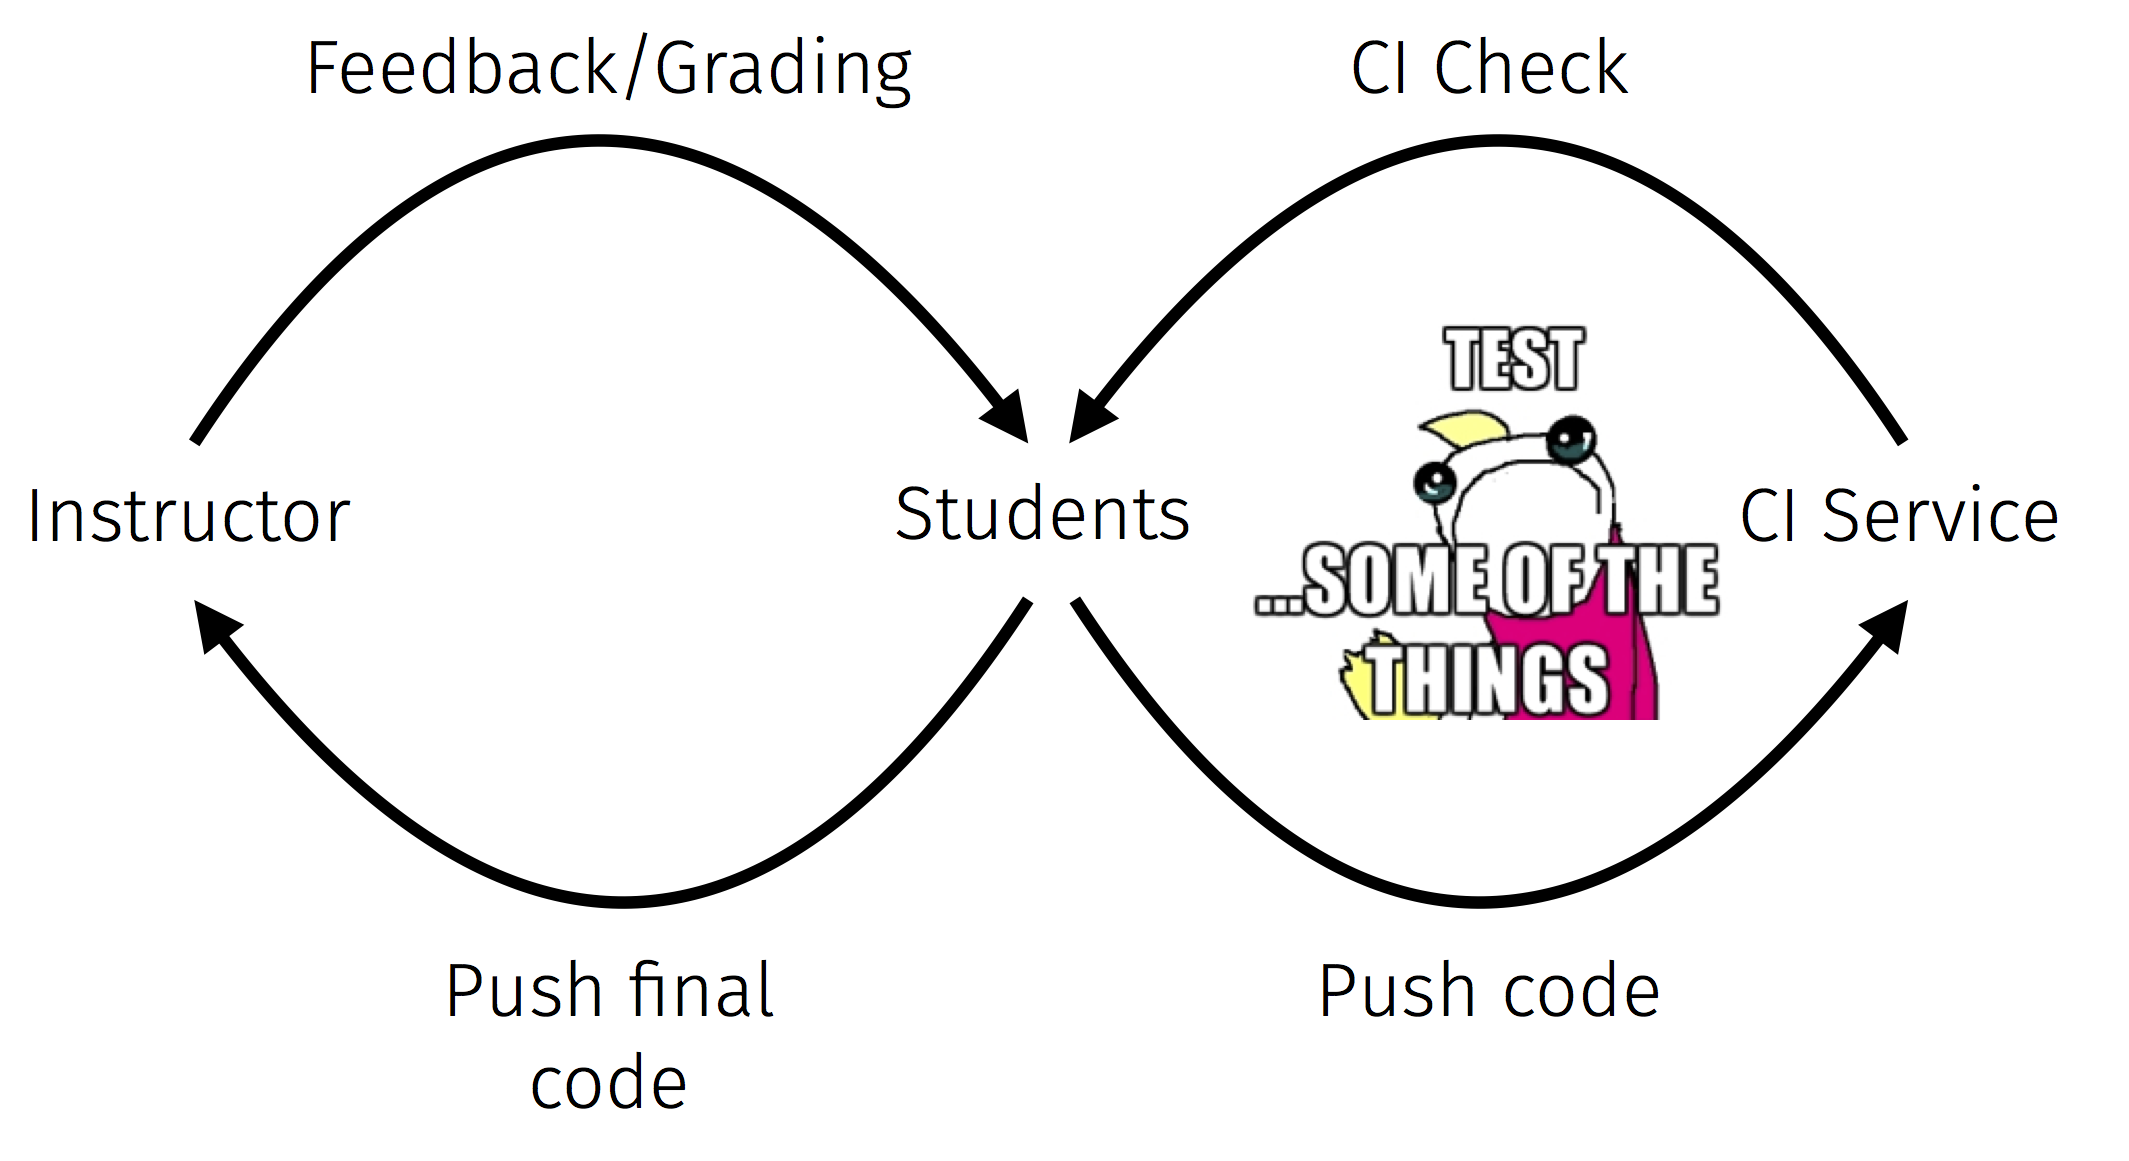
\includegraphics[width=\textwidth]{imgs/cycle_ci_meme.png}}
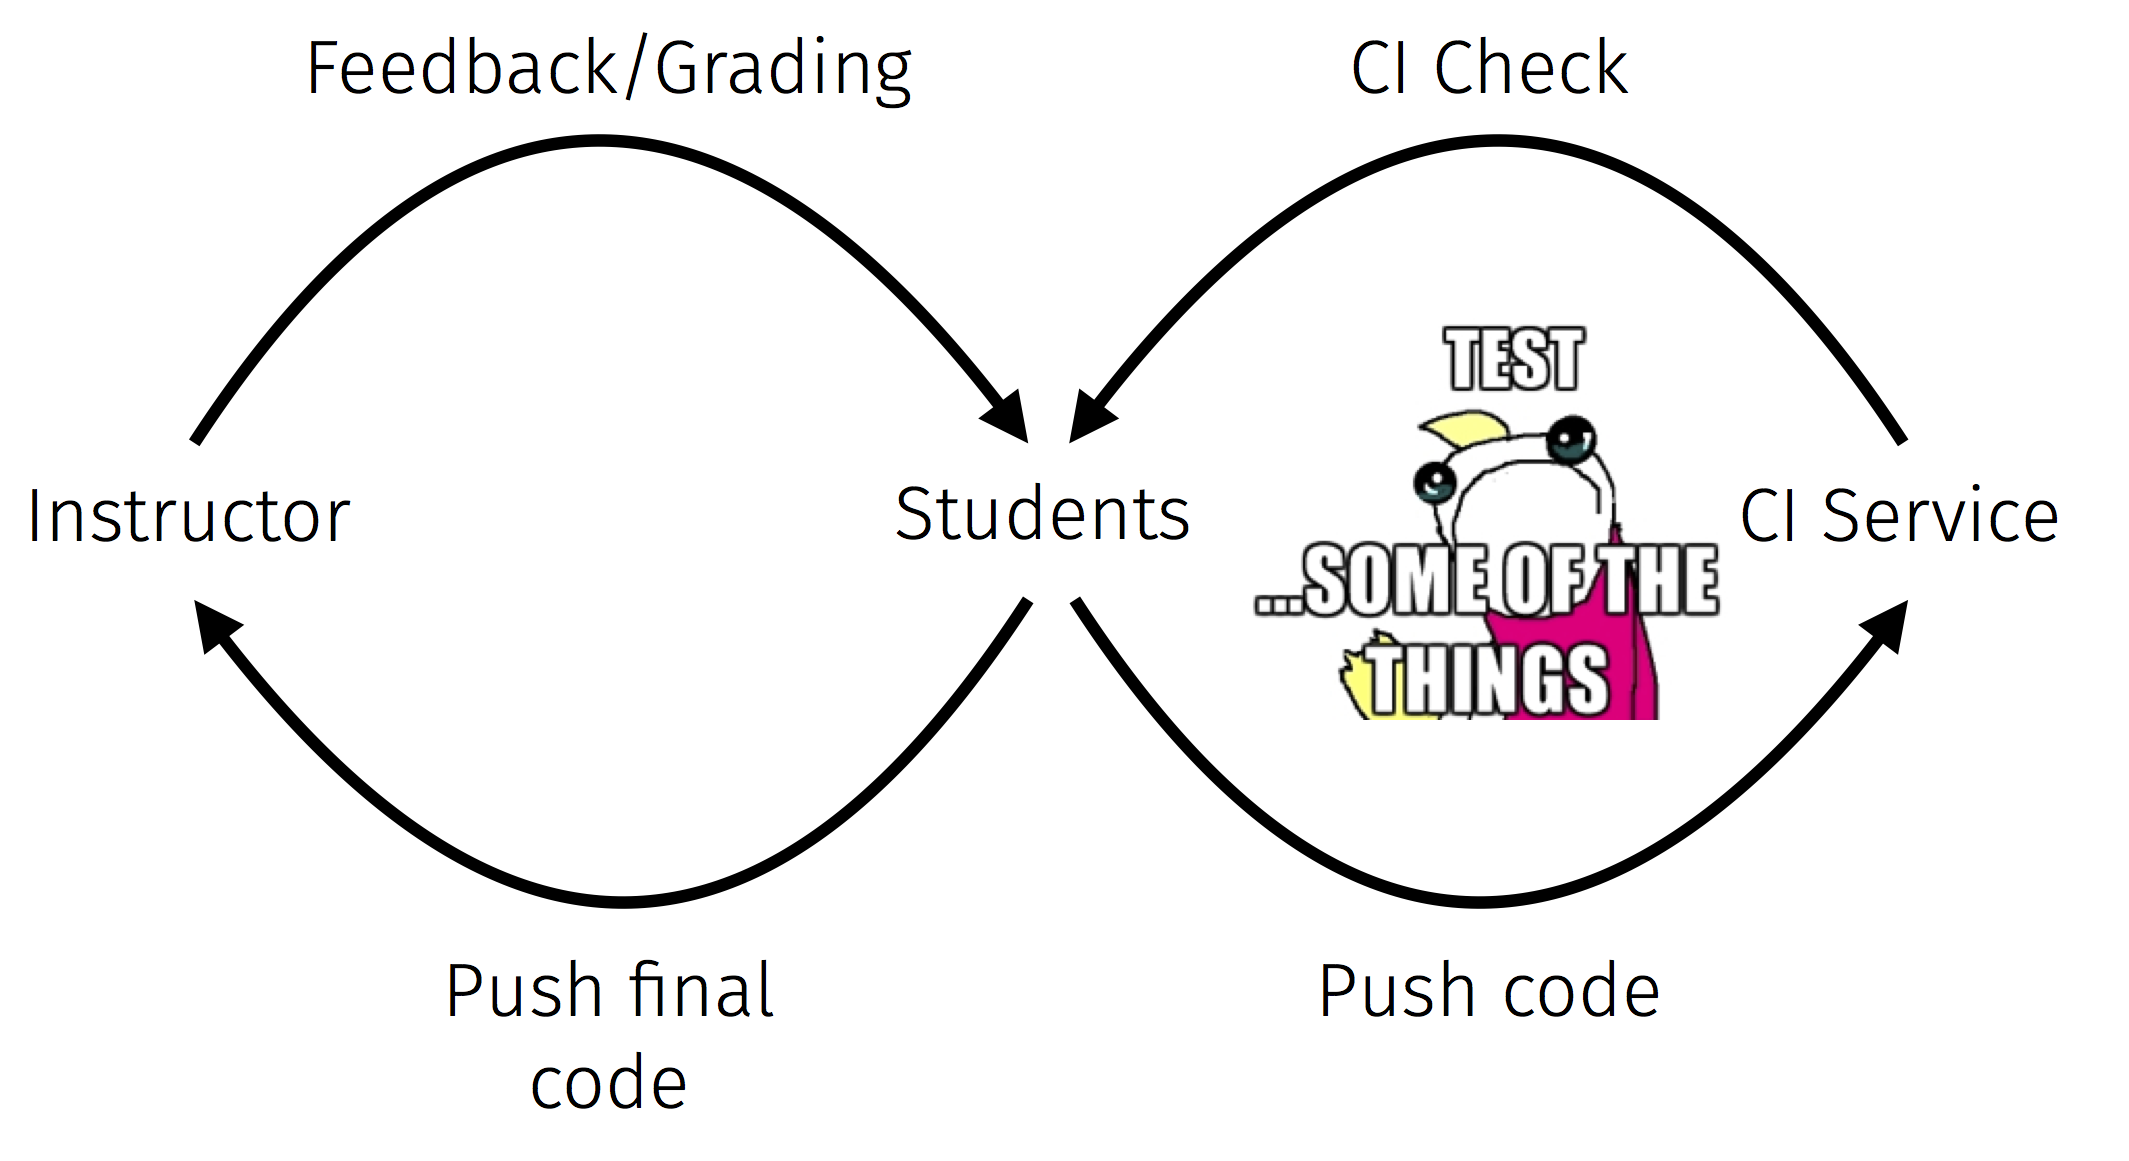
\includegraphics[width=\textwidth]{imgs/cycle_ci_meme.png}
\end{center}

Goal is not to test for correctness - test for process / reproducibility.

\end{frame}

%%%%%%%%%%%%%%%%%%%%%%%%%%%%%%%%%%%%%%%%%%%%%%%%%%%%%%%%%%%%%%%%%%%%%%%%%%%%%%


\begin{frame}
\frametitle{Wercker}

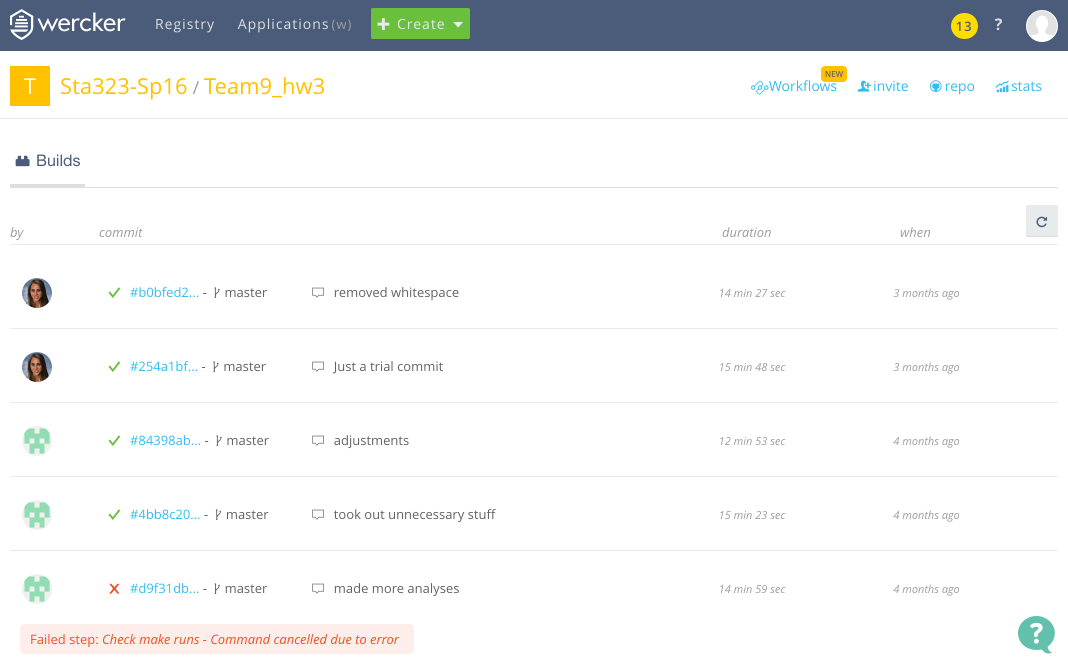
\includegraphics[width=\textwidth]{imgs/wercker_builds.png}
    
\end{frame}

%%%%%%%%%%%%%%%%%%%%%%%%%%%%%%%%%%%%%%%%%%%%%%%%%%%%%%%%%%%%%%%%%%%%%%%%%%%%%%

\begin{frame}
\frametitle{Wercker Steps}

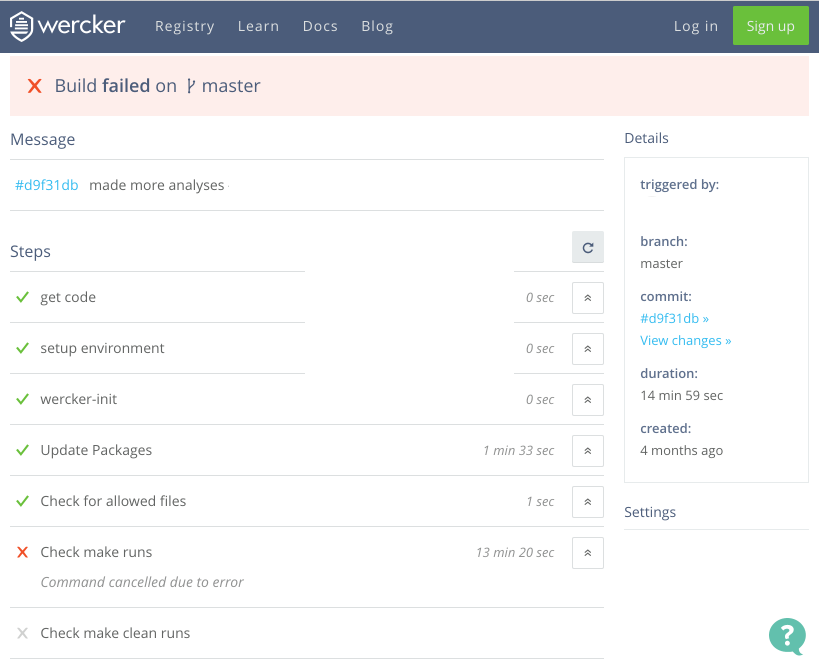
\includegraphics[width=\textwidth]{imgs/wercker_fail.png}

\end{frame}

%%%%%%%%%%%%%%%%%%%%%%%%%%%%%%%%%%%%%%%%%%%%%%%%%%%%%%%%%%%%%%%%%%%%%%%%%%%%%%

\begin{frame}
\frametitle{Wercker Error}
\begin{center}
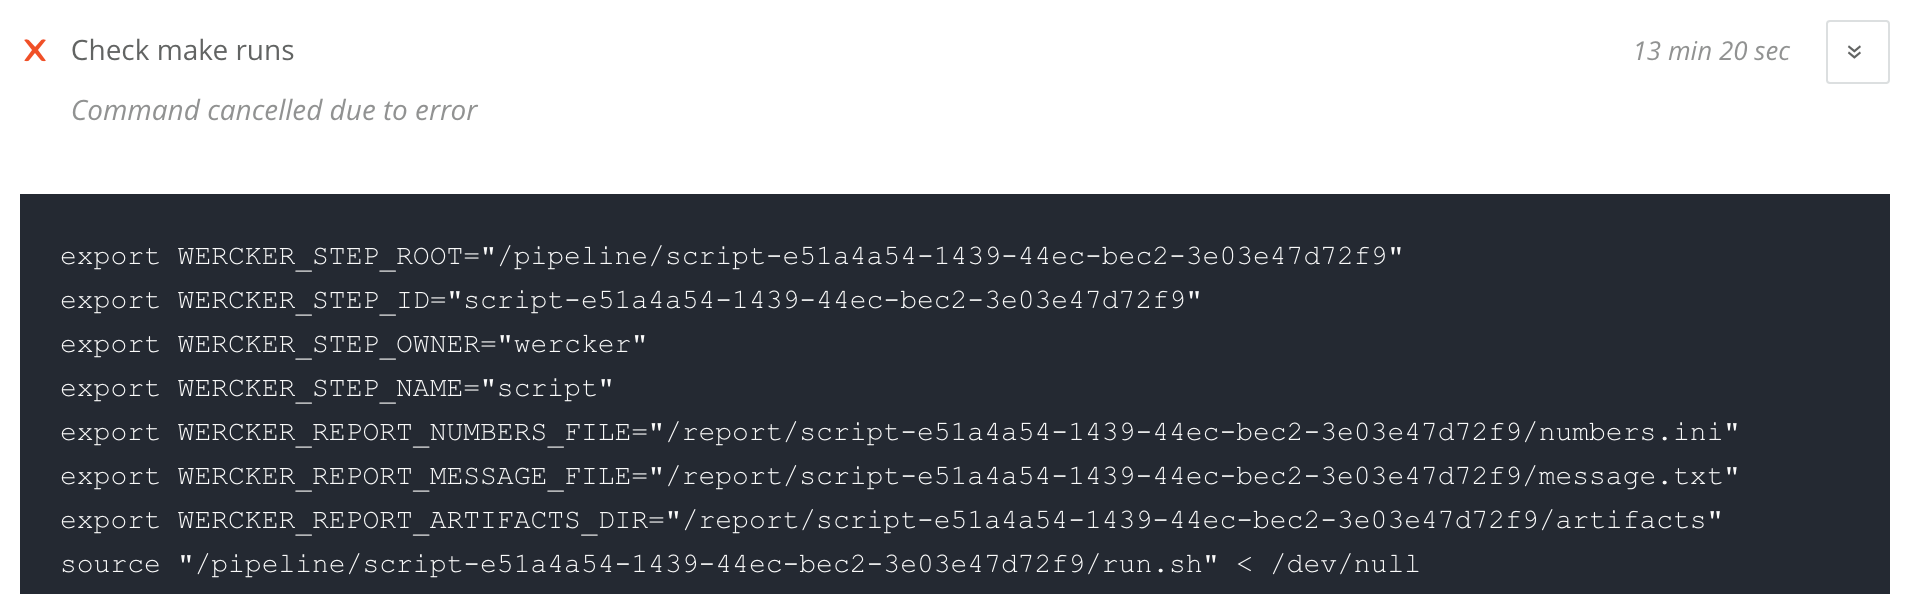
\includegraphics[width=\textwidth]{imgs/wercker_error1.png} \\
$\vdots$ \\
\vspace{1mm}
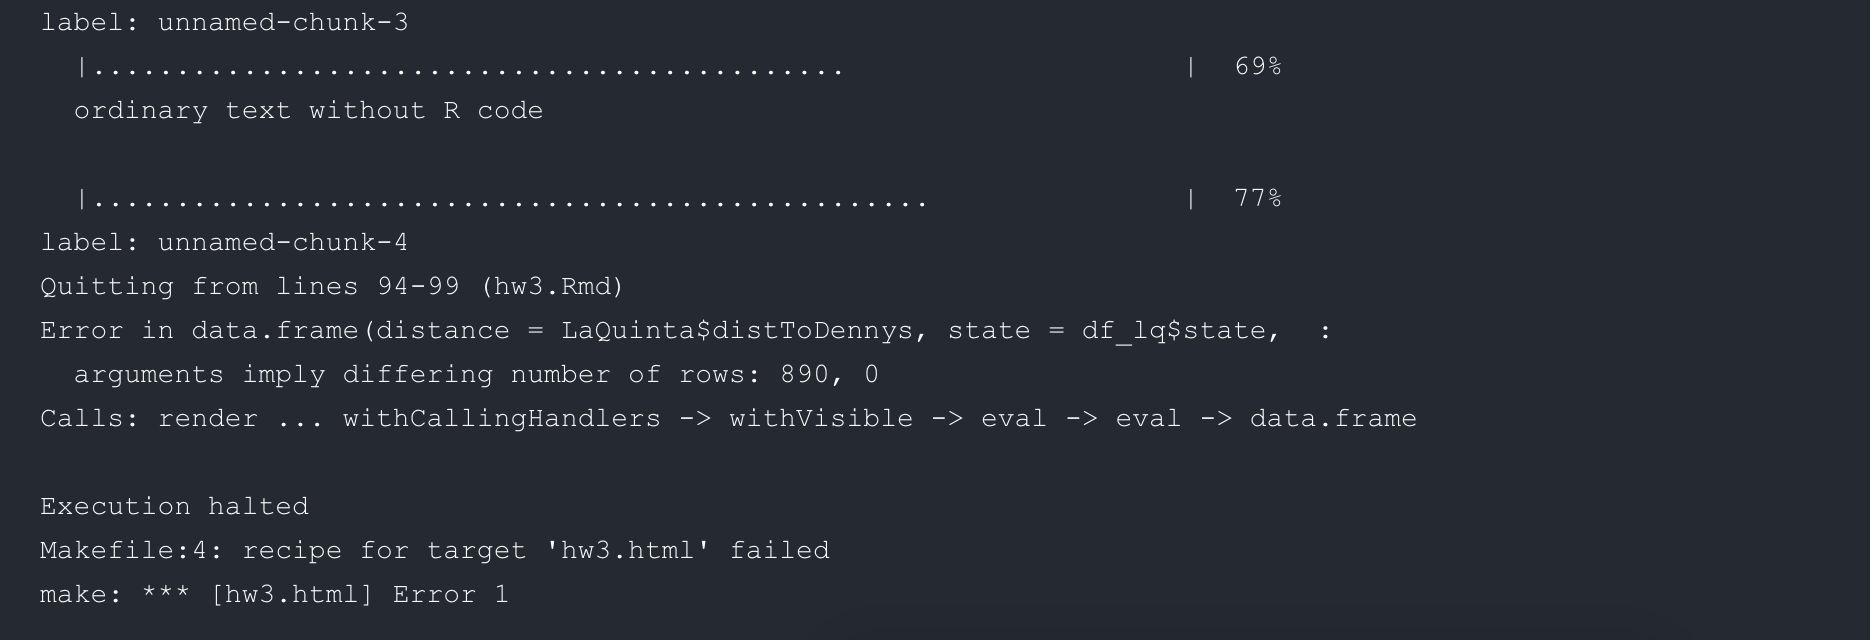
\includegraphics[width=0.98\textwidth]{imgs/wercker_error2.png}
\end{center}
\end{frame}

%%%%%%%%%%%%%%%%%%%%%%%%%%%%%%%%%%%%%%%%%%%%%%%%%%%%%%%%%%%%%%%%%%%%%%%%%%%%%%

\begin{frame}[t]
\frametitle{Final Analysis}

\vspace{-2mm}

\makebox[\linewidth][c]{

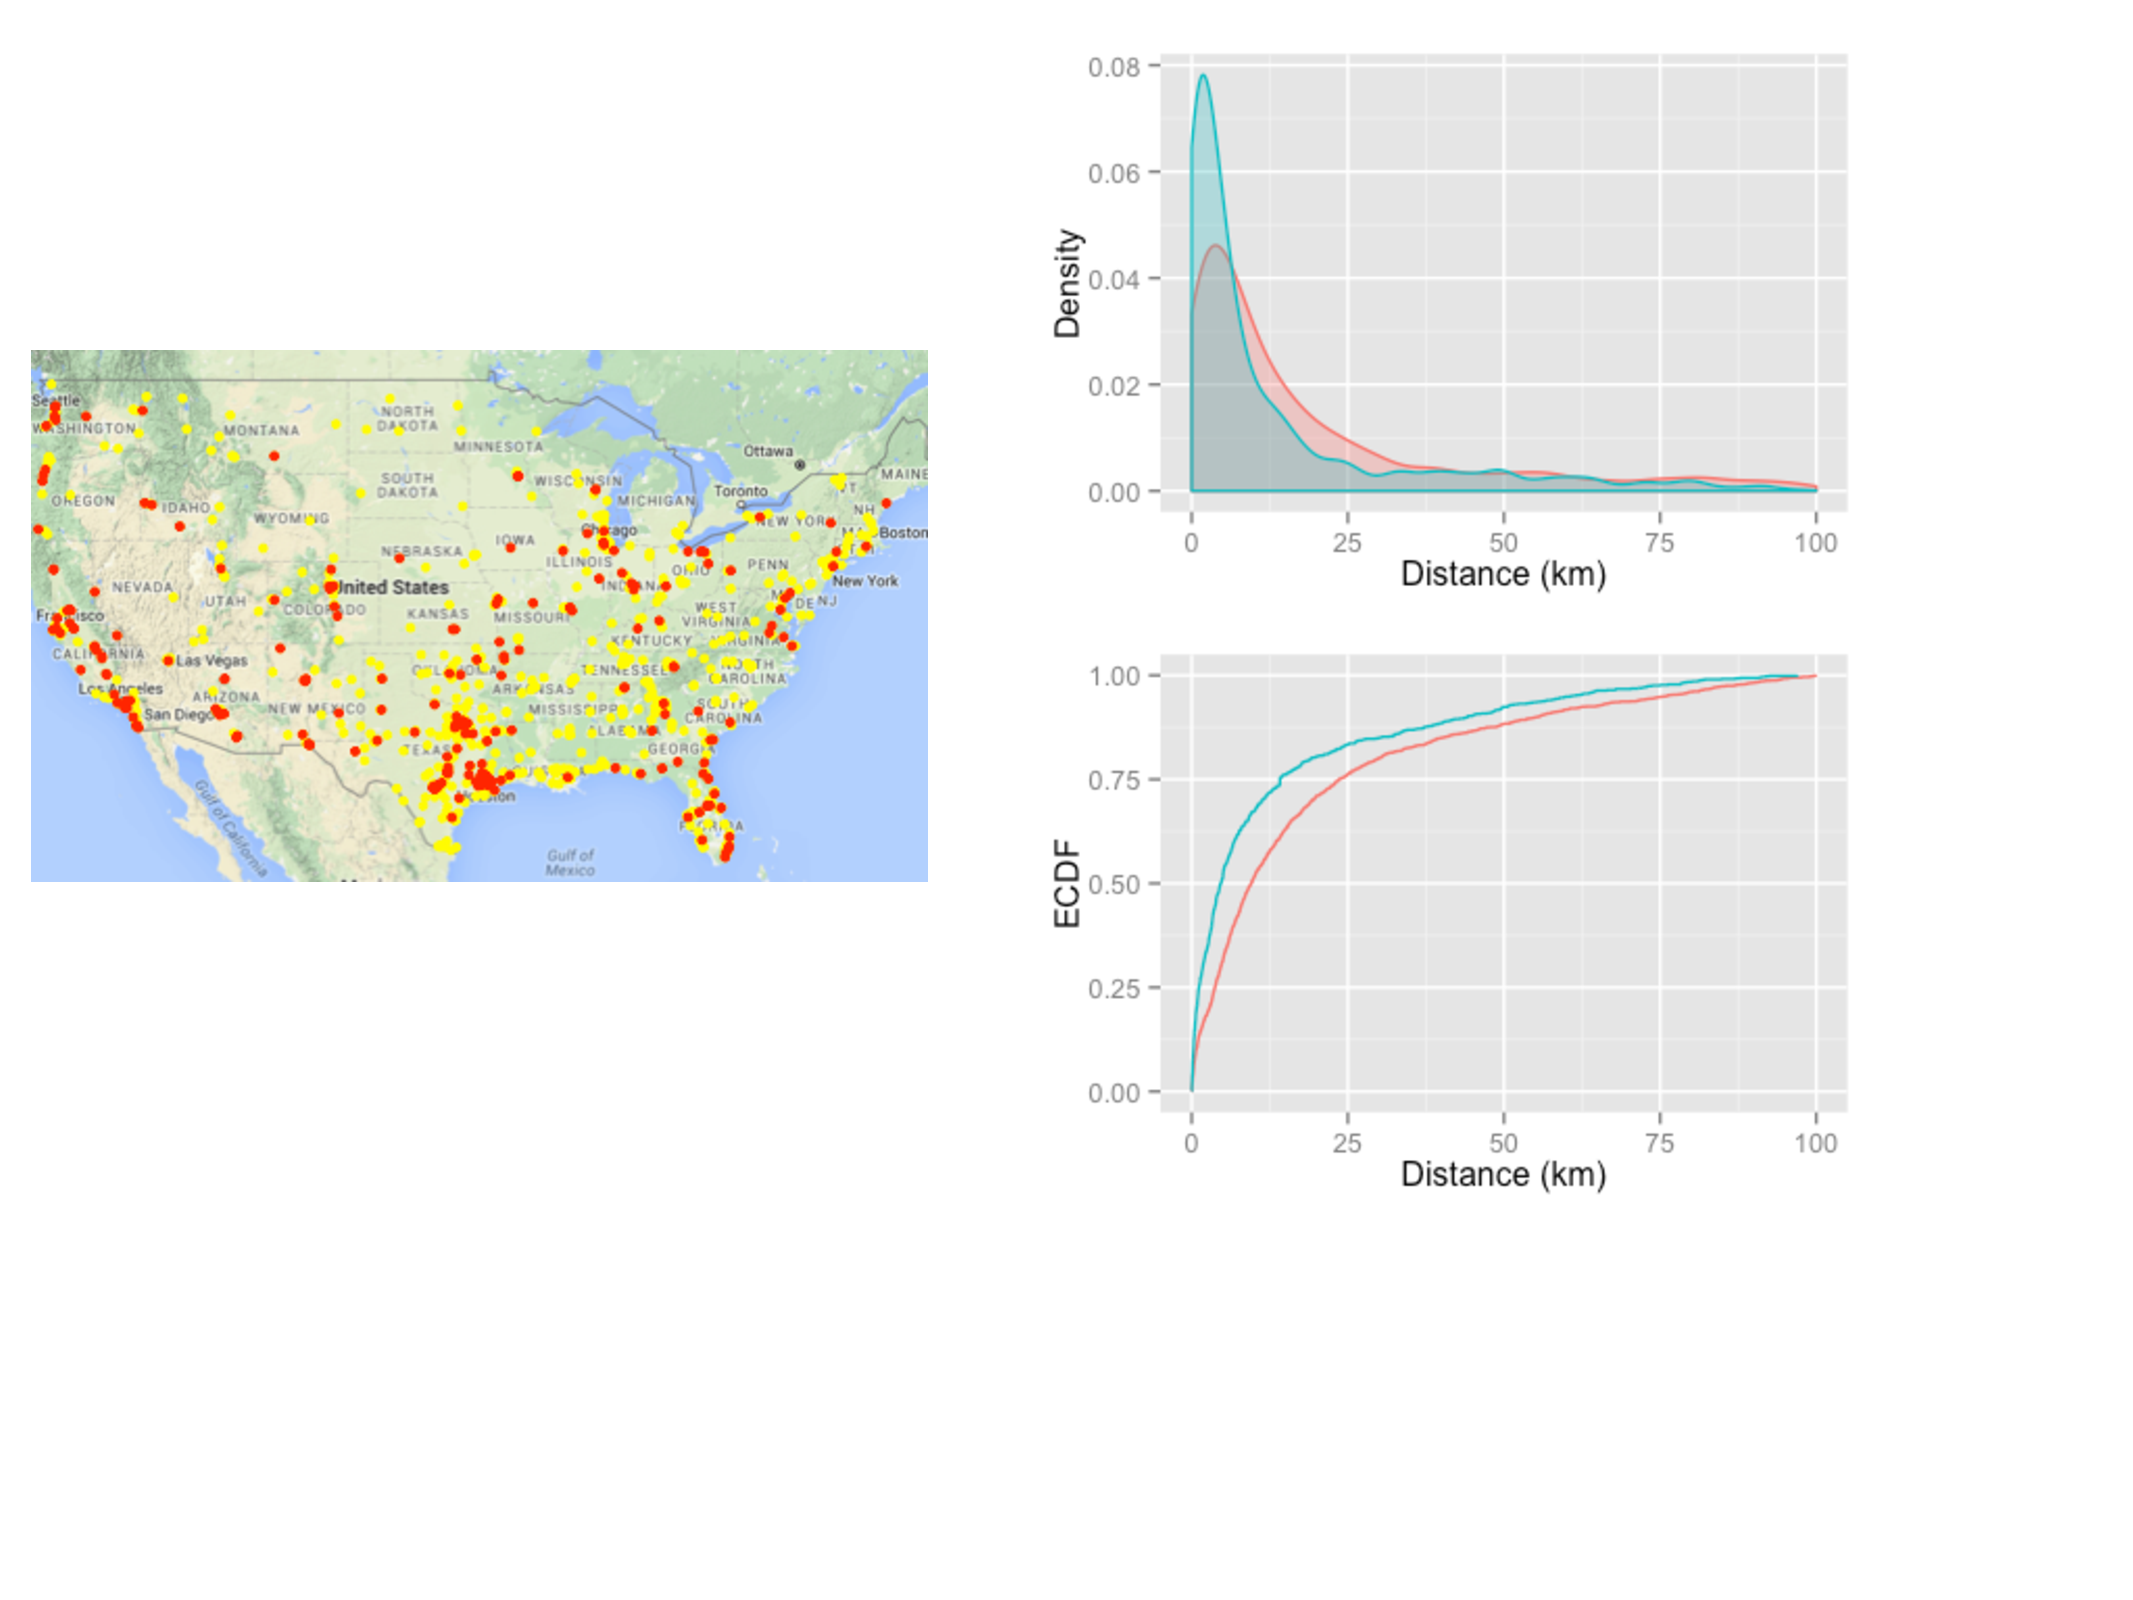
\includegraphics[width=1.1\textwidth]{imgs/dennys_lq_results.pdf}

}

\end{frame}


%%%%%%%%%%%%%%%%%%%%%%%%%%%%%%%%%%%%%%%%%%%%%%%%%%%%%%%%%%%%%%%%%%%%%%%%%%%%%%

\begin{frame}[t]
\frametitle{Lessons Learned}

\begin{itemize}
\item Use github$^*$ for everything
\vspace{4mm}
\item Investments in automation pay off 
\vspace{4mm}
\item Don't reinvent the wheel - borrow software engineering best practices
\vspace{4mm}
\item Programming fundamentals are important - but tools and applications provide better motivation
\vspace{4mm}
\end{itemize}

\end{frame}

%%%%%%%%%%%%%%%%%%%%%%%%%%%%%%%%%%%%%%%%%%%%%%%%%%%%%%%%%%%%%%%%%%%%%%%%%%%%%%


\begin{frame}[t]
\frametitle{Questions, Comments?}

\begin{center}
{\small
%\renewcommand*\arraystretch{2.5}
\begin{tabular}{ll}
\raisebox{-0.3\height}{
\includegraphics[width=0.3in]{imgs/email_icon.png}}  & rundel@gmail.com \\
\\
\raisebox{-0.3\height}{
\includegraphics[width=0.3in]{imgs/github_icon.png}} & github.com/rundel/ \\
\\
\raisebox{-0.3\height}{
\includegraphics[width=0.3in]{imgs/pres_icon.png}}   & github.com/rundel/Presentations/ \\
\\
\raisebox{-0.3\height}{
\includegraphics[width=0.3in]{imgs/home_icon.png}}   & bit.ly/Sta523\_2014 \\ 
                                                                            & bit.ly/Sta523\_2015 \\
                                                                            & bit.ly/Sta323\_2016 \\
\end{tabular}
}
\end{center}

\end{frame}



\end{document}








